\begin{wrapfigure}{r}{0.4\textwidth}
  \vspace{-0.3in}
  \centering
  \begin{minipage}[t]{\linewidth}
    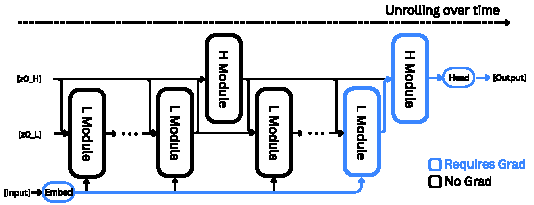
\includegraphics[width=\linewidth]{figures/pseudocode/HRMDiagram.pdf}
    \begin{lstlisting}[language=python]
def hrm(z, x, N=2, T=2):
    x = input_embedding(x)
    zH, zL = z

    with torch.no_grad():
        for _i in range(N * T - 1):
            zL = L_net(zL, zH, x)
            if (_i + 1) % T == 0:
                zH = H_net(zH, zL)

    # 1-step grad
    zL = L_net(zL, zH, x)
    zH = H_net(zH, zL)
    return (zH, zL), output_head(zH)

# Deep Supervision
for x, y_true in train_dataloader:
    z = z_init
    for step in range(N_supervision):
        z, y_hat = hrm(z, x)
        
        loss = softmax_cross_entropy(y_hat, y_true)
        z = z.detach()

        loss.backward()
        opt.step()
        opt.zero_grad()
    \end{lstlisting}
  \end{minipage}
  \vspace{-0.15in}
  \caption{\textbf{Top:} Diagram of HRM with approximate gradient. \textbf{Bottom:} Pseudocode of HRM with deep supervision training in PyTorch.}
  \label{fig:pseudocode}
\end{wrapfigure}